%\documentclass[preprint1,12pt]{aastex}
\documentclass[]{article}

%=====================================================================
% CUSTOM: PACKAGES, MACROS \& SETTINGS
%=====================================================================

% packages for figures
\usepackage{graphicx}
%\usepackage{psfig,epsfig}
% packages for symbols
%\usepackage{latexsym,amssymb}
% AMS-LaTeX package for e.g. subequations
%\usepackage[fleqn]{amsmath}
\usepackage{amsmath}
\usepackage{todonotes}
% citation style
\usepackage{natbib}
\citestyle{aa}
\usepackage[colorlinks=true,linkcolor=blue,citecolor=blue]{hyperref}
%\usepackage[backend=bibtex, style=authoryear-icomp, sortlocale=de_DE, natbib=true, url=false, doi=true, eprint=false]{biblatex}
%\addbibresource{RefBib.bib}
%\renewcommand*{\bibfont}{\footnotesize}
%\renewbibmacro{in:}{}
%\AtEveryBibitem{\clearfield{title}}


%=====================================================================
% FRONT MATTER
%=====================================================================

\slugcomment{Draft \today}
%\slugcomment{Submitted to ApJ}

\shorttitle{How BH physics fails in Illustirs}

\shortauthors{Gonz\'alez-Casanova et al.}

%=====================================================================
% BEGIN DOCUMENT
%=====================================================================

\begin{document}

\author{Diego F. Gonz\'alez-Casanova\altaffilmark{}, Tim Haines, Brianna Smart, Andrea Vang, Zachary Peace}
\altaffiltext{}{Astronomy Department, University of Wisconsin-Madison, 475 North Charter Street, Madison, WI 53706-1582, USA}



\title{How BH physics fails in Illustirs}

\begin{abstract} 
Bla bla ... we are great. 
\\ 
\end{abstract}

\keywords{black hole physics, accretion, numerical - cosmology}

%===============================================
%===============================================

\section{Introduction} 

\subsection{Black Hole Properties in the Illustrious Simulation}
Accreting black holes (BHs) such as active galactic nuclei (AGN) are believed to be important in the evolution of galaxies as the feedback from AGN can trigger and/or quench star formation. Thus, in order to understand galaxy evolution, it is important to understand the physics of BH. Specifically, it's important to probe the BH's influence on its surrounding environment.\\

There are distinctive signatures of BH activity that can be used to probe the existence of BH. For example, relativistic jets emitting synchrotron radiation in the radio band are one signature. Strong X-ray emission from from inverse-Compton scattering in the corona can be related to the accretion flow of the BH. In 2003, \citet{Merloni2003}  investigated the properties of $\sim$100 AGN's compact emission in the X-ray and radio bands and showed that the radio luminosity is correlated with both the mass and the X-ray luminosity at a highly significant level. These sources defined a fundamental plane in the three-dimensional space as shown in Figure \ref{FP}. The fundamental plane (FP) suggests that the physical processes regulating the conversion of an accretion flow into radiative energy could be universal across the entire black hole mass scale \citep{Merloni2003}. The FP is defined as:

\begin{equation}
\log L_R=0.6 \log L_x+0.78 \log M+7.33 \; ,
\end{equation}

where the radio luminosity is $L_R$, the X-ray luminosity is $L_X$, and the mass of the BH is $M$.Then from the FP, the accretion-powered X-ray luminosity can be expressed as: 

\begin{equation}
\log L_x = \log M+q \log \dot{m}+K_2  \; ,
\label{LxFP}
\end{equation}

where $K_2$ is normalization constant. Depending on the accretion flow model, the efficiency coefficient $q$ ranges from 0.5 (optically thick thin disk accretion flow) to 2.3 (advection dominated accretion flow). The most significant aspect of the FP is that it is a correlation which we can apply our general knowledge of galactic BHs to AGNs and vice versa.\\

\begin{figure}
\centering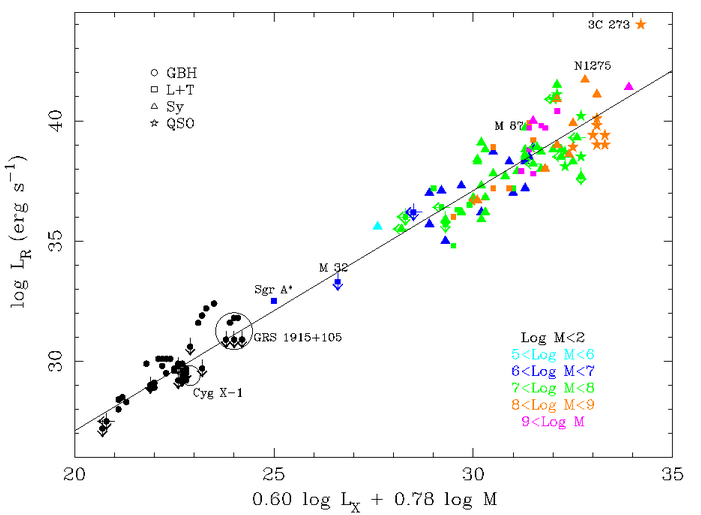
\includegraphics[height=0.6\linewidth,clip=true]{./Figures/FP.png}
\caption{Edge-on view of the fundamental plane given by the BH mass, radio luminosity, and X-ray luminosity. \label{FP}}
\end{figure}

\subsection{Black Holes in the Illustris Simulation}

The Illustris Project is a series of large-scale cosmological hydrodynamical simulations of galaxy formation \citep{Vogelsberg2014}. The simulation consists of large cosmological situations in a periodic box with 106.5 Mpc, simulated with different physics at different resolutions. It assumes a standard flat $\Lambda$CDM cosmology with $\Omega_{m,0}=0.2726$, $\Omega_{\Lambda,0}=0.72746$, $\Omega_{b,0}=0.0456$, and $H_{0}=70.4$ km s$^{-1}$ Mpc$^{-1}$ from the Wilkinson Microwave Anisotropy Probe 9-year data realease \citep{Hinshaw2013}. \\

In the Illustris simulations, collision-less black hole particles with a seed mass of $1.42 \times 10^5 M_\odot$ are placed in dark matter halos of mass greater than $7.1 \times 10^10 M_\odot$ \citep{Sijacki2014}.  The black hole seeds are allowed to grow through gas accretion or through mergers with other black holes.  At $z=0$, there are 32,542 black holes in total with 3965 black holes more massive than $10^7 M_\odot$ \citep{Sijacki2014}. \\

In our project, we aim to reproduce the fundamental plane of black hole activity in the Illustris Project to see how well the BHs in the simulation fit with observations. Most specifically, we aim to determine the efficiency coefficient $q$ in Equation \ref{LxFP} in the Illustris simulation using the mass and mass accretion rates of BHs. From this analysis, we can begin to understand to how well the Illustris simulates the real physics of black holes in the universe.\\

This paper is structured as follows. In Section~\ref{sec:dis} we discuss our results in accordance to the Illustris simulations and the fundamental plane of BH. In Section~\ref{sec:con} we give our conclusions.

\section{Discusion and Results} \label{sec:dis}

The BH population in Illustris was analysed using the low resolution simulation at a red shift of $z = 0$.  The Illustris simulation gives the mass and accretion rate for each BH.  We first eliminate all BH particles with $M = 0$ or $\dot{M} = 0$, which we assume to be unphysical. We will hereafter refer to the remaining population (admittedly somewhat anomalously) as the �Full Illustris-2 Black Hole Sample�. Analysing those two properties for the whole sample set we found there are some BH with really low accretion rates (\ref{fig:bhpop_full}).  Since we are attempting to fit a linear relationship effectively between mass an accretion rate, such anomalously low-accreting black holes should be omitted. \\

\begin{figure}[]
\centering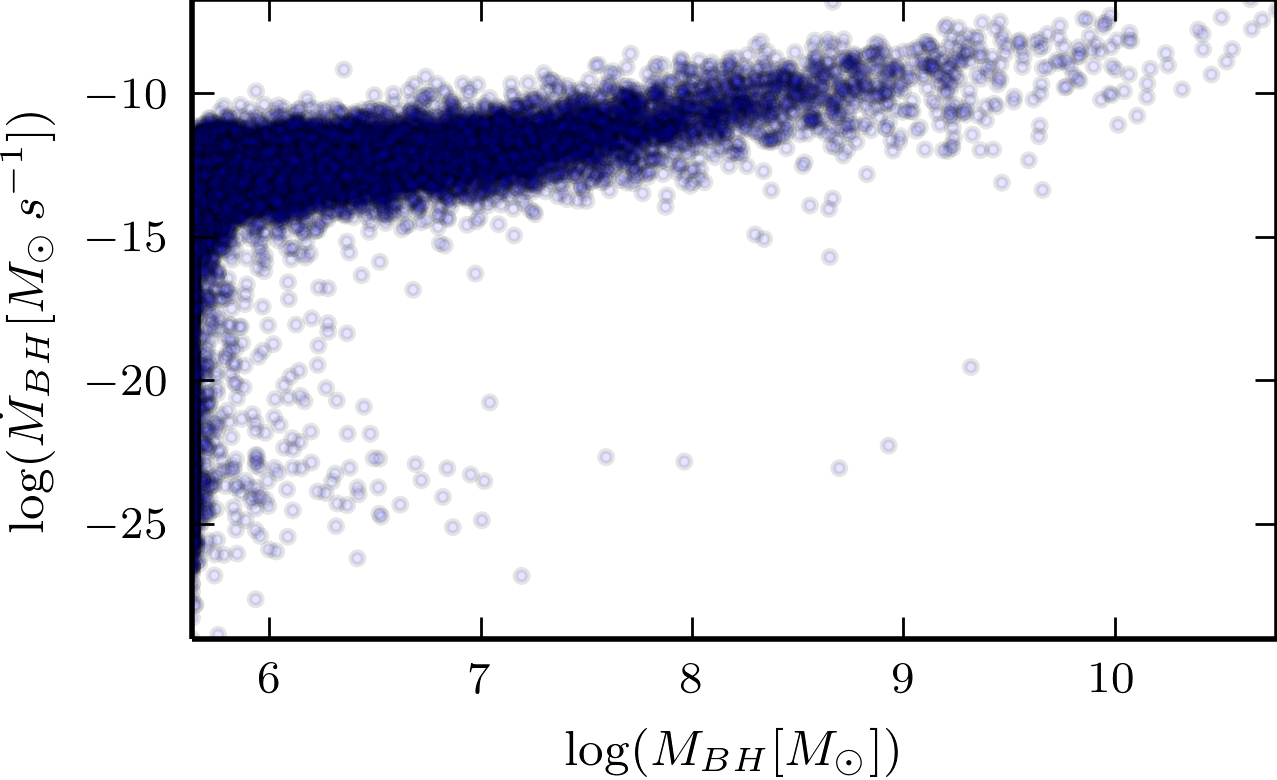
\includegraphics[height=0.6\linewidth,clip=true]{./Figures/Illustris2_bhpop_full.png}
\caption{Each light blue dot represents a single black hole. Two populations are apparent: a quiescent group and a much larger accreting population.}
\label{fig:bhpop_full}
\end{figure}

We accomplished this by first noting that the main sequence of black holes follows roughly a log-normal distribution in accretion rate space, centered around approximately $\dot{M}_{BH} = 10^{-12.5} M_{\odot}/s$. However, there also exists a small, secondary population centered around approximately $\dot{M}_{BH} = 10^{-15.7} M\odot/s$ (see \ref{fig:bhpop_mdot}). To effectively eliminate the low-accreting BHs, we impose a hard lower limit on accretion rates, and eliminate all data below that cutoff.\\

\begin{figure}[]
\centering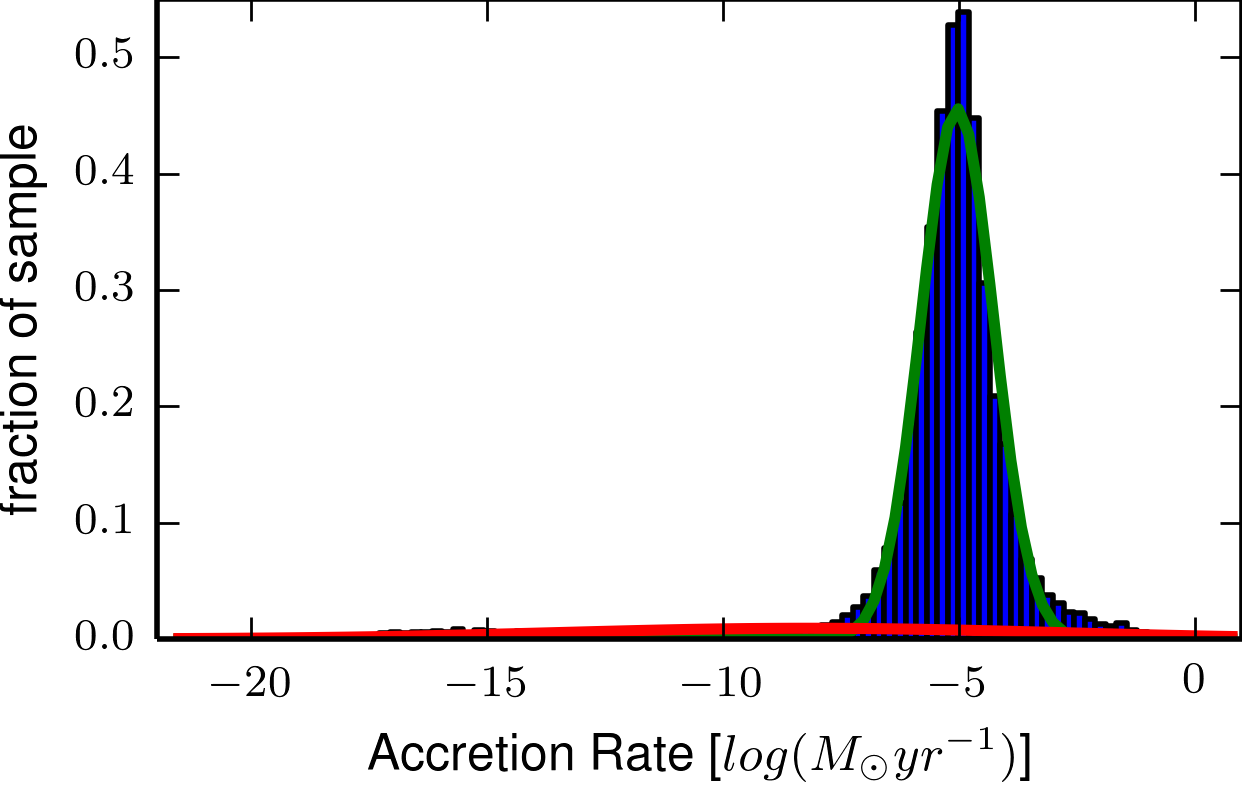
\includegraphics[height=0.6\linewidth,clip=true]{./Figures/Illustris2_bhpop_mdot.png}
\caption{The Full Sample exhibits a weak, but noticeable bimodality in accretion rate space. We fit two log-normal distributions to the raw distribution, and impose a strict cutoff on the accretion rate, eliminating most of the anomalously low-accreting population.}
\label{fig:bhpop_mdot}
\end{figure}

With the low-accreting black holes eliminated , we can then construct a power-law relationship between $M$ and $\dot{M}$ using linear least-squares (Figure \ref{fig:bhpop_hist2d}). The best-fit found is:

\begin{equation}
 log_{10}(\dot{M}) = 0.569 log_{10}(M) - 17.855 \;.
\label{eq:int_relation}
\end{equation}

This relationship reflects the intrinsic properties of the simulation, and is subject to no additional models.\\

\begin{figure*}
\begin{center}
\leavevmode
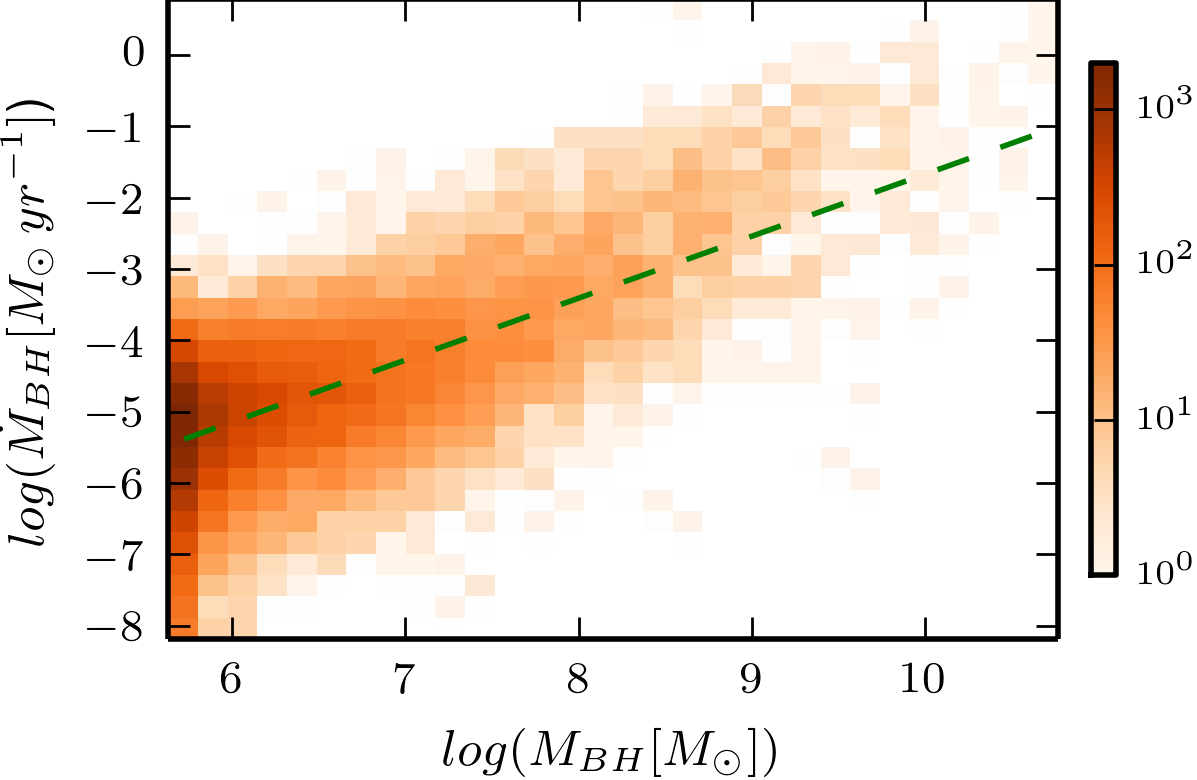
\includegraphics[height=0.6\linewidth,clip=true]{./Figures/Illustris2_bhpop_hist2d.png}
\caption{The best-fit power-law relationship between $M$ and $\dot{M}$ for the sample of Illustris-2 BHs, after imposing an accretion rate threshold. The fit is overlaid onto a histogram of the same population, and fifty of the sample�s data points.}
\label{fig:bhpop_hist2d}
\end{center}
\end{figure*}


Figure \ref{fig:bhpop_hist2d} demonstrates that the vast majority of black holes in Illustris-2 are low-mass and low-accretting. However, it is interesting to note that the observed accretion rates of the entire population are much too low to account for their observed mass. For example, a typical low-mass ($10^7 M_{\odot}$) black hole accretes at approximately $10^{-12} M_\odot s^{-1}$. This implies that the accretion rate for these black holes must have been much higher in the past, to account for the mass observed now (multiplying the current accretion rate of such a black hole by the simulation time yields an accreted mass of $\sim 10^{5} M_{\odot}$. A similar result holds for the high-mass, high-accreting black holes (for which $\dot{M} \sim 10^{-10} M_{\odot}/s$ yields a constant-accreted mass $\sim 10^{7} M_{\odot}$, compared the the observed mass $\sim 10^{9} M_{\odot}$).\\

The fundamental plane of the BH�s relates the mass, X-ray luminosity and accretion rate.  Because the luminosity is not an intrinsic property of the simulation, it had to be calculated.  The calculation of the luminosity for BH can be approximated by two different models.  The first one takes into account the Eddington luminosity of the BH, which relates it to the mass, and the second uses the thin disk approximation, which relates the luminosity to the accretion rate.  Both of these approximations for the luminosity gives the bolometric luminosity. To get the X-ray luminosity from the bolometric luminosity we use the Elvis data sample to calculate a template \citep[][Figure \ref{fig:Elvis_template}]{elvis}. The equation relation from the Elvis template is given by:

\begin{equation}
L_x =0.1947 L_{bol} + 1.656\times 10^{-15} \;.
\end{equation}

\begin{figure}[]
\centering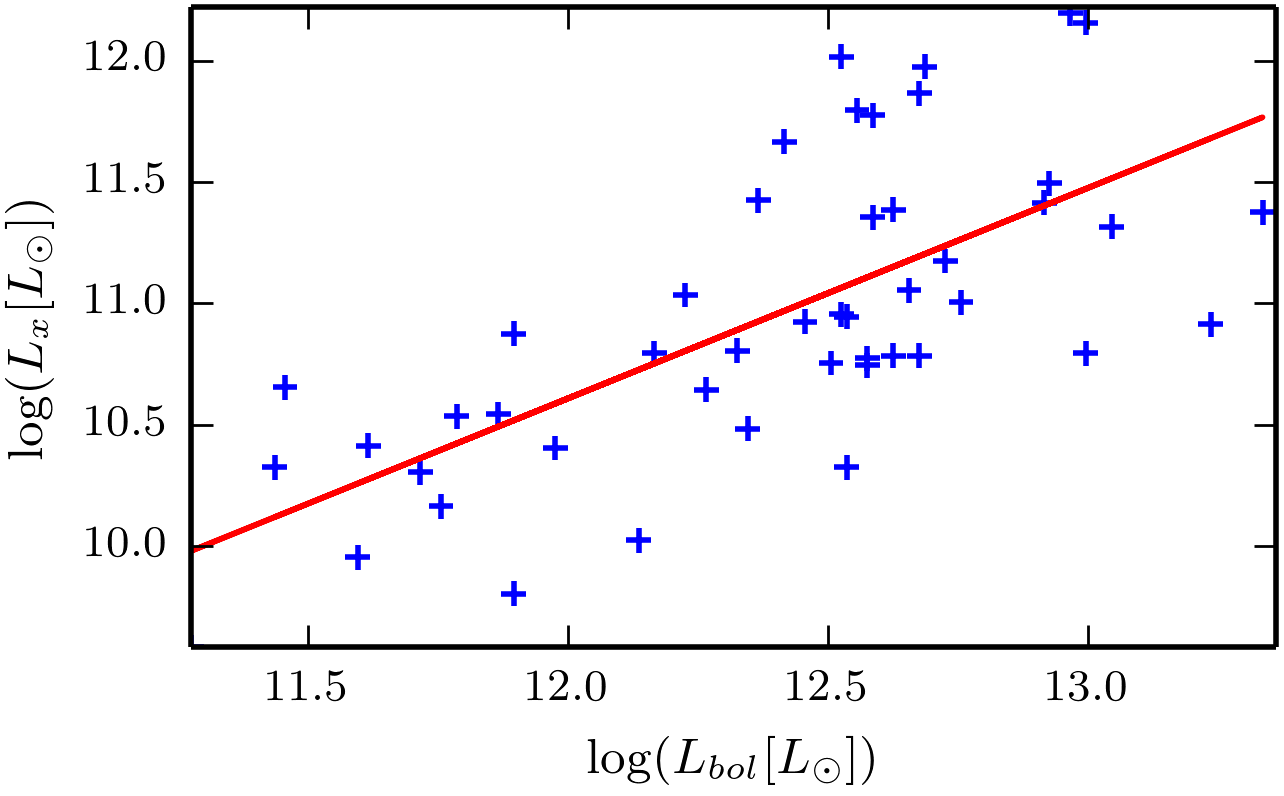
\includegraphics[height=0.6\linewidth,clip=true]{./Figures/elvis_template.png}
\caption{The data points from the \citet{elvis} BH luminosities over plot with the best-fit linear relation between $L_x$ and $L_{bol}$ for the sample.}
\label{fig:Elvis_template}
\end{figure}

Assuming the BH is only emitting at 10\% off the Eddington luminosity and by means of the Elvis Template the X-luminosity for the BH is:

\begin{equation}
L_x =623.04 M + 1.656\times 10^{-15} \;.
\label{eq:Lx_propto_m}
\end{equation}

By assuming a thin disk approximation with 10\% efficiency we get that the X-luminosity for the BH is:

\begin{equation}
L_x =4.64\times 10^{19} \dot{M} + 1.656\times 10^{-15} \;,
\label{eq:Lx_propto_mdot}
\end{equation}

for all the cases the masses, accretion rates and luminosities are measured in $M_{\odot}$,   $M_{\odot} s^{-1}$ and $L_{\odot}$.  With equations \ref{eq:Lx_propto_m} and \ref{eq:Lx_propto_mdot} and using the equation \ref{LxFP}.  The fundamental plane equation can be rewritten in terms of mass, accretion rate, k and q.  By means of using the intrinsic mass to accretion relation, equation \ref{eq:int_relation}, the fundamental plane can be express with only 3 variables. 

\begin{multline}
 log_{10}(9.03\times 10^{18} \dot{M} + 1.656\times 10^{-15})  + 1.115 log_{10}(\dot{M})\\
  - \frac{e}{d} q log_{10}(\dot{M}) + k = 0 
 \end{multline}
 \begin{multline}
log_{10}(623.04 + \frac{1.656\times 10^{-15}}{M})\\
 - 0.869 q log_{10}(M) +17.855 -k = 0        
\end{multline}

The parameter $q$ holds the information on the properties of the BH.  Hence the adequate value that fits the simulations had to be found.  Using the Newton-Raphson numerical root-finding method for the two equations and evaluating throw the whole data sample, $q$ is express in terms of $k$. \\

By means of this analysis, we found that there is a high correlation between the values of $q$ and $k$. Since we hope to reproduce the slope $q$ from \citet{Merloni2003}, which does not provide typical values for $k$, we must approach this in a rather roundabout manner. We assume that both approximations for $L_x$ are equally good, and will yield similar results, and combine \ref{eq:Lx_propto_m} and \ref{eq:Lx_propto_mdot} with the relationship found between $M$ and $\dot{M}$:

\begin{multline*}
log_{10}(a_1 + \frac{b}{M}) - d q log_{10}(M) + e q\\
 - log_{10}(a_2 \dot{M} + b)  + \frac{1}{d} log_{10}(\dot{M}) - \frac{e}{d} q log_{10}(\dot{M}) = 0\;,
\label{q_equation}
\end{multline*}

where $a_1$, $a_2$, and $b$ are obtained from converting simulation units to physical units; and $d$ and $e$ are the slope and the intercept of the power-law found above. The constants have the following values:

\begin{itemize}
%these need units!
\item $a_1 = 623.04$
\item $a_2 = 9.03 \times 10^{18}$
\item $b = 1.656 \times 10^{-15}$
\item $d = 0.869$
\item $e\footnote{Any resemblance to a mathematical constant is unintentional. Sorry.} = -17.855$
\end{itemize}

A value of $q$ is found for each black hole by inputting values of $M$ and $\dot{M}$, and solving for $q$ using Newton-Raphson numerical root-finding. For the distribution of black holes in our Illustris-2 sample, the distribution of $q$ values is shown in \ref{fig:q_nr_hist}. The distribution of $q$ values obtained is strongly peaked at around $.068$, with a mean of $.0693$.

%\begin{figure}
%\centering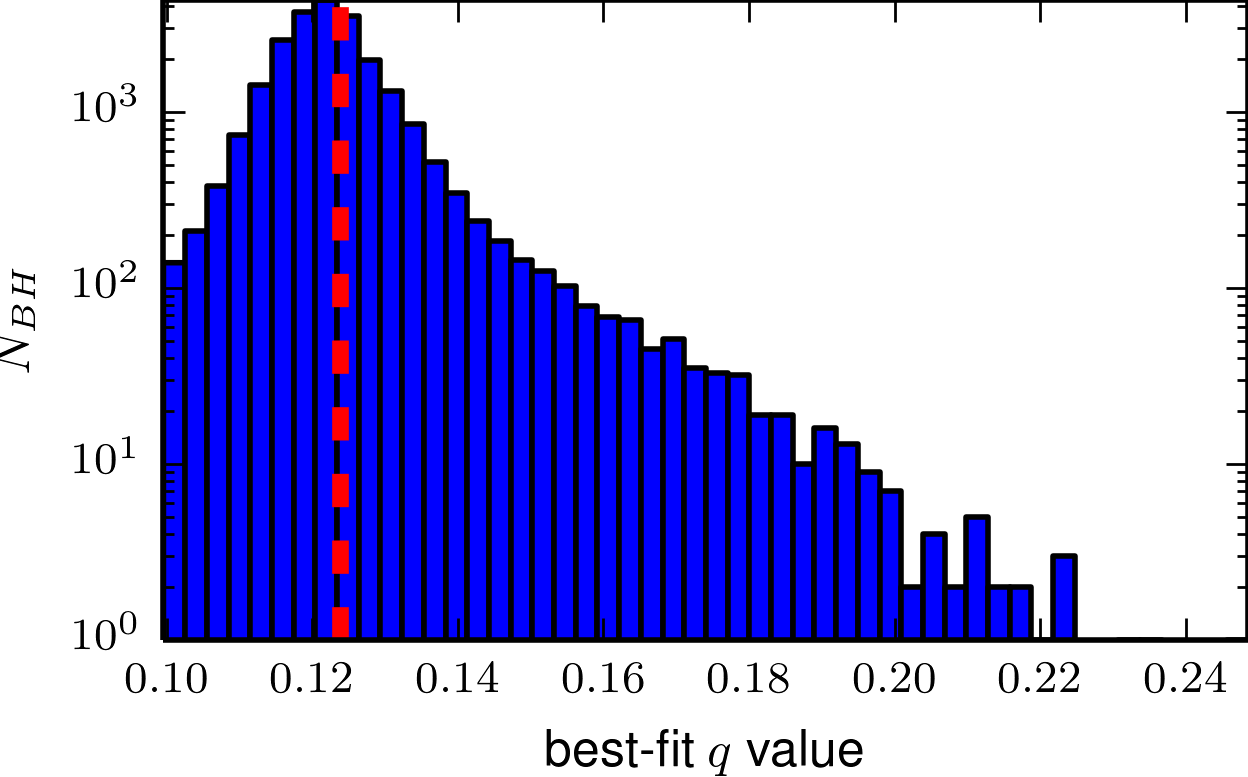
\includegraphics[height=0.6\linewidth,clip=true]{./Figures/q_nr_hist.png}
%\caption{A log-histogram of the number of best-fit $q$ values, with one value found per Illustris-2 black hole, using Newton-Raphson root finding. The maximum likelihood is (SOMEWHERE), with (SOME NUMBER OF) black holes, and the mean value is $0.693$.}
%\label{fig:q_nr_hist}
%\end{figure}

%here we�ll want to do some statistics on the distribution of the q values: something like 86/14 limits might work well: I (Zach) work on this and make a new figure.




\section{Conclusions} \label{sec:con}

%\bibliography{example}
%\bibliographystyle{apj}
%\bibliography{RefBib}
%\begin{thebibliography}{58}
%\bibitem[Merloni2003]{Merloni2003} Merloni 2003, apj, 222, 22
%\bibitem[Hinshaw2013]{Hinshaw2013} Merloni 2003, apj, 222, 22
%\bibitem[Vogelsberg2014]{Vogelsberg2014} Merloni 2003, apj, 222, 22
%\bibitem[Sijacki2014]{Sijacki2014} Merloni 2003, apj, 222, 22
%\bibitem[Elvis]{elvis} Merloni 2003, apj, 222, 22
%\end{thebibliography}

\end{document}

